\chapter{Experimental Details}

Having discussed all of the relevant theoretical aspects of the Higgs boson and its role in the Standard Model as 
well as how we can measure it in particle colliders in theory, it is now necessary to explain how this is done in 
practice. This chapter covers all experimental tools used to do so relevant to this thesis, from the Large Hadron 
Collider (LHC) that facilitates particle collisions to the ATLAS detector that records their interaction products. 
I will start with discussions about the hardware of the LHC and ATLAS and then move on to talk about object 
reconstructions within the context of our experiment.

\section{The Large Hadron Collider}

The Large Hadron Collider (LHC) is the largest proton-proton collider in the world, located at the CERN
\footnote{"Organisation européenne pour la recherche nucléaire" or in its english translation "European 
Organization for Nuclear Research"} laboratory near Geneva, Switzerland. It is a circular collider with a circumference 
of 26.7 km and can accelerate both protons and heavy ion beams to $6.8\ TeV$, leading to center of mass energies of up 
to $13.6\ TeV$ in collisions. To facilitate these collisions, the LHC accelerates two collimated beams \footnote{The 
beams are not continuous but rather consist of individual bunches that are spaced evenly} of hadrons simultaneously and 
guides them towards each other at 4 intersection points (bunch crossings) at rates of up to 40 MHz. These points 
correspond to the sites of the four main detectors located on the LHC ring: ATLAS, CMS, LHCb and ALICE. \par

%https://www.nature.com/articles/s42254-024-00758-5
\begin{figure}
\centering
    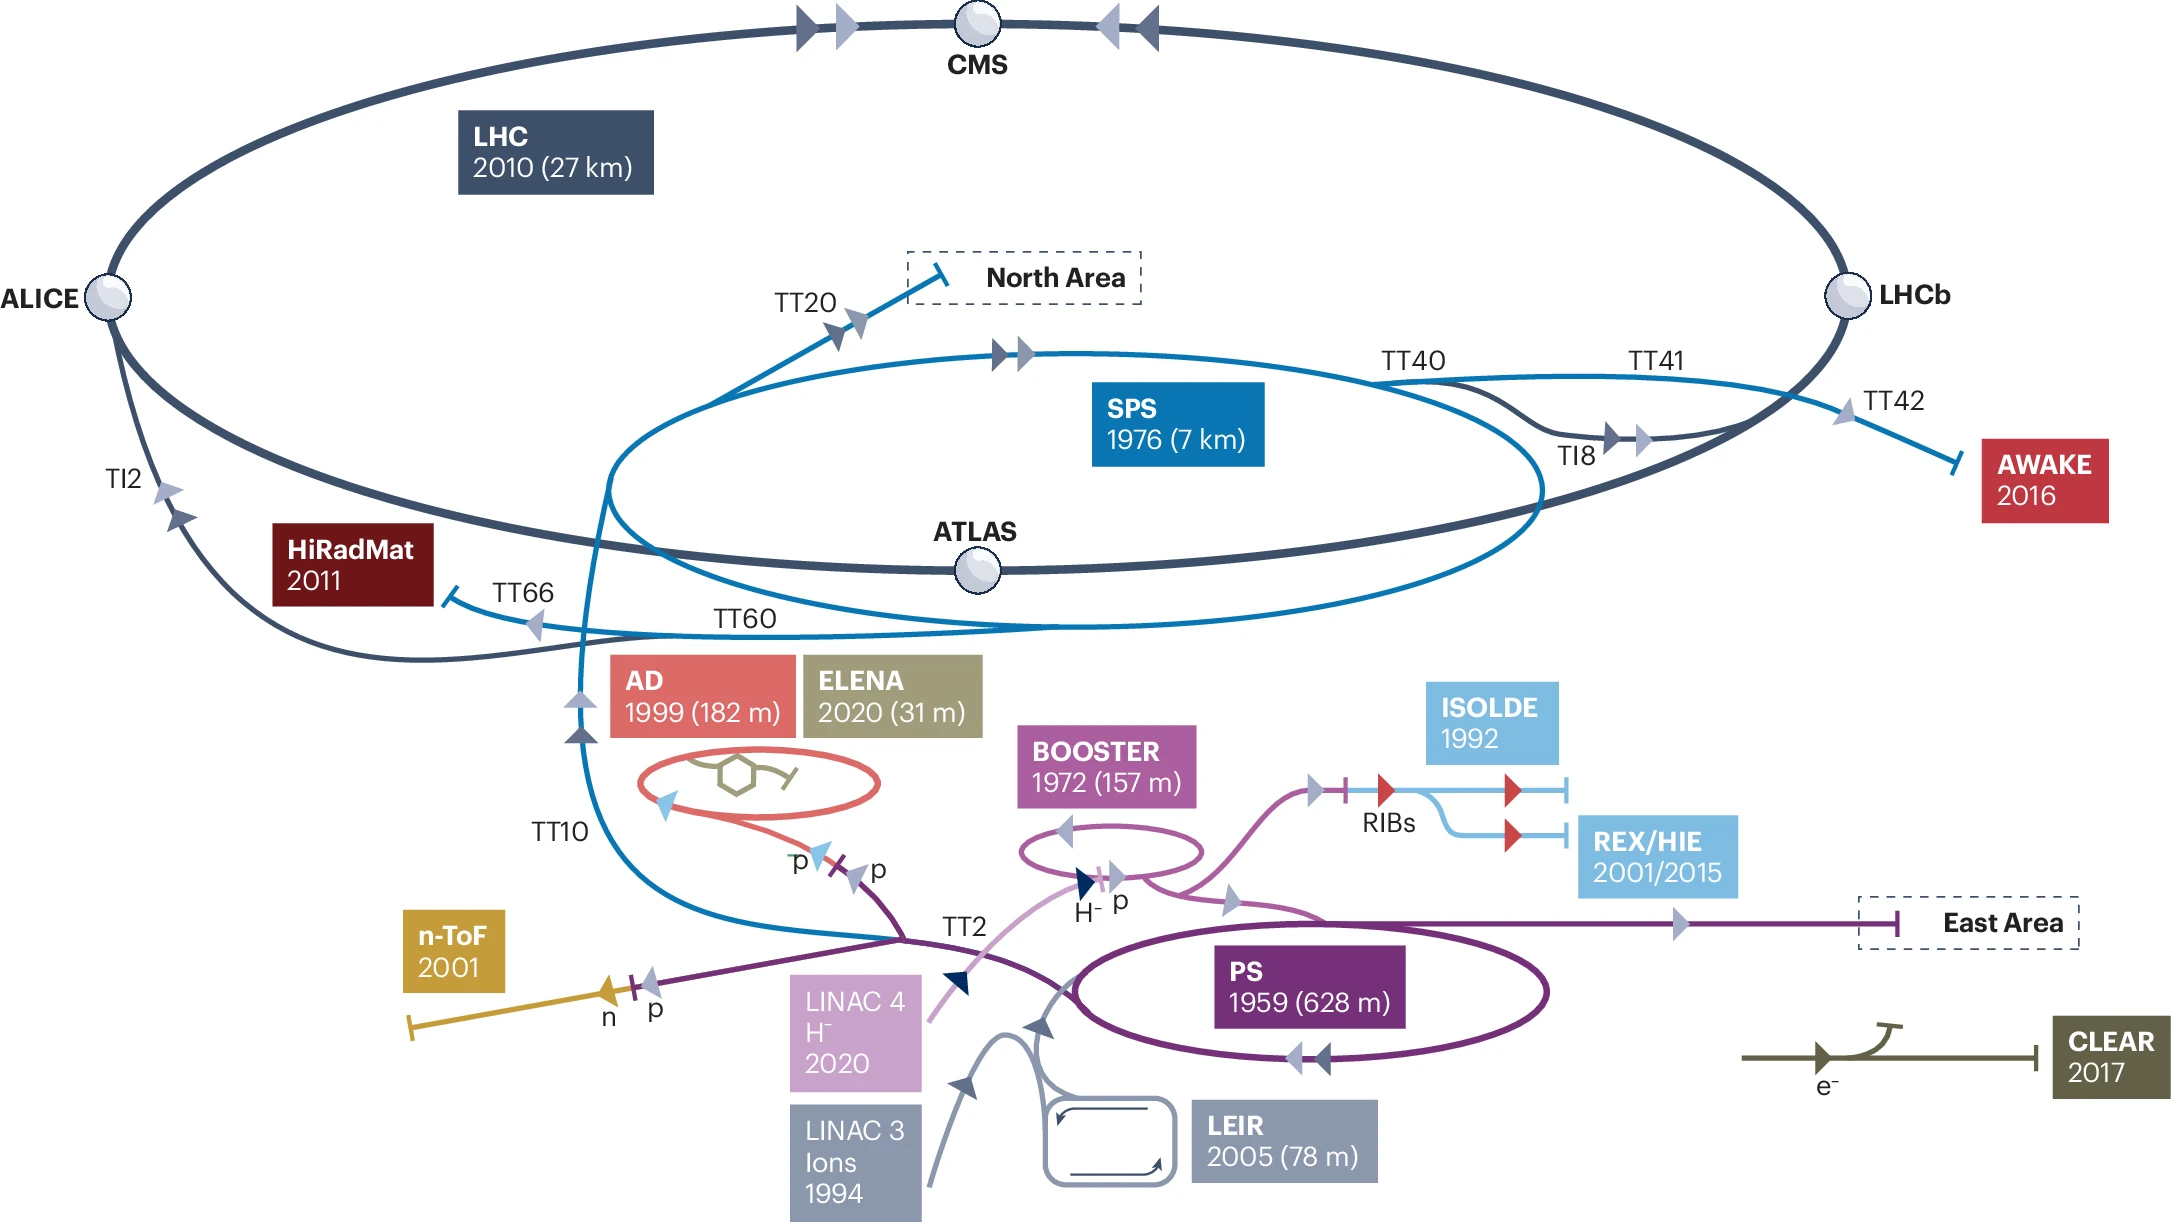
\includegraphics[width=1.0\textwidth]{images/CERN_Complex.png}
    \caption{Schematic overview of the CERN accelerator complex including main synchrotron accelerators LHC, SPS 
    and PS.}
    \label{fig:CERN_Complex}
\end{figure}

Achieving the desired collision energies requires the use of mutliple components of the CERN accelerator complex 
detailed in figure \ref{fig:CERN_Complex}, which consists of linear and smaller circular colliders that were operated 
as independent experiments in the past. The acceleration is facilitated by an intricate setup of magnets (mostly 
dipoles and quadrupoles), 
which also steer and focus the beams. For proton-proton collisions this process starts with $H^-$ ions which are 
accelerated to $160\ MeV$ by a linear accelerator called Linac4. From there the ions are injected into the circular  
Proton Synchrotron Booster (PSB), which strips both electrons from the Hydrogen ions and creates a pure proton beam with 
an energy of $2\ GeV$. Afterwards the beam is accelerated to $26\ GeV$ by the Proton Synchrotron (PS) and $450\ GeV$ by the Super Proton Synchrotron (SPS) before finally being injected into the LHC where it reaches its final collision energy. 
\par

%https://home.cern/news/news/accelerators/accelerator-report-excellent-2024-lhc-run-ended-abruptly
\begin{table}
\begin{center}
\caption{Overview of run periods of the LHC between 2008 and 2026.}
\label{table-lhc-runs}
\begin{tabular}{|c c c c|} 
 \hline
 Run Number & Years & Center of mass energy & Integrated Luminosity \\ [0.5ex] 
 \hline
 1 & 2008-2013 & $7-8\ TeV$ & $29.2\ fb^{-1}$ \\ 
 2 & 2015-2018 & $13\ TeV$ & $159.8\ fb^{-1}$ \\ 
 3 & 2022-2026 & $13.6\ TeV$ & $195.9\ fb^{-1}$ (up to and including 2024) \\ 
 \hline
\end{tabular}
\end{center}
\end{table}

The LHC has been operational since 2008, when it recorded its first proton-proton collisions at a center of mass energy 
of $7\ TeV$. Operation has been split into three distinct run periods denoted runs 1, 2 and 3 with shutdowns in 
between for maintenance and accelerator upgrades. Details on the timeline of these runs, alongside achieved energy and 
luminosity is shown in table \ref{table-lhc-runs}. Run 1 is mostly relevant for historical reasons and this thesis will 
focus on data collected during runs 2 and 3 given the much higher center of mass energy. The LHC presents the backdrop 
for the research of thousands of physicists spread across the ATLAS, CMS, ALICE and LHCb collaborations as well as 
multiple smaller teams at any given time. It is the best tool we have available to study the kinds of most fundamental 
particle interactions we are interested in.

\section{The ATLAS Detector}

ATLAS (\textbf{A} \textbf{T}oroidal \textbf{L}HC \textbf{A}pparatu\textbf{S}) is the largest of the four main detectors 
around the LHC ring. It is a general purpose detector designed to record the proton-proton collision signatures 
generated in LHC collisions without focusing too heavily on any specific processes, requiring trade-offs in detector 
design. It is around 46 meters long with a diameter of 25 meters and weights 7000 tons. The detector, visualized in 
figure \ref{fig:ATLAS_Detector}, consists of four main active components: an inner tracking detector, a calorimeter 
system and a muon spectrometer. Each of these components interacts differently with different types of particles, as 
summarized in figure \ref{fig:Detector_Interactions}. The inner tracking detector is responsible for precise trajectory 
measurements of charged particles and represents the most intricate part of the ATLAS detector. The calorimeter system 
is used to measure the energy of electrons and photons (electromagnetic calorimeter) as well as hadrons (hadronic 
calorimeter). Finally the muon system identifies muons penetrating the rest of the detector. In order to make accurate 
measurements of particle momentum, the ATLAS detector uses a magnet system to curve the trajectories of charged 
particles. All of these elements will be discussed in more detail in this section.

%https://cerncourier.com/a/atlas-undergoes-some-delicate-gymnastics/
\begin{figure}[h!]
\centering
    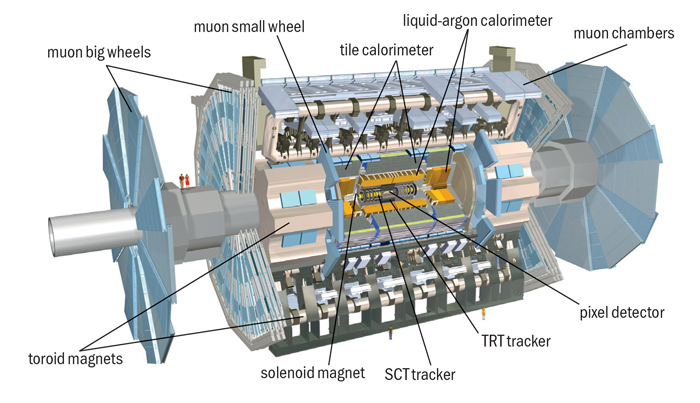
\includegraphics[width=0.8\textwidth]{images/ATLAS_Detector.jpg}
    \caption{Diagram showing all components of the ATLAS detector.}
    \label{fig:ATLAS_Detector}
\end{figure}

%https://www.nbi.dk/~petersen/Teaching/Stat2011/Project1/project1.html
\begin{figure}
\centering
    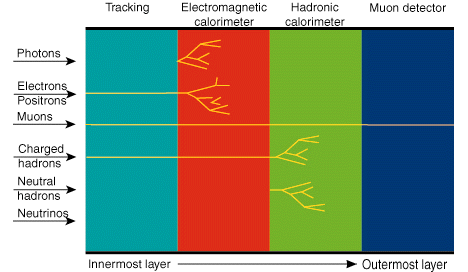
\includegraphics[width=0.8\textwidth]{images/Detector_Interactions.png}
    \caption{Sketch showing how different particles interact with detector components.}
    \label{fig:Detector_Interactions}
\end{figure}

\subsection{ATLAS Coordinate System}

Before diving into the detail of the various detector components, it is important to establish the coordinate system 
used in the ATLAS experiment as well as survey physical quantities of interest related to the measurement and 
reconstruction of particle trajectories. By convention, the coordinate system is centered at the collision point, with 
the beam line representing the z-axis, the x-axis pointing towards the center of the ring and the y-axis pointing 
towards the sky, as seen in figure \ref{fig:ATLAS_Coordinate_System}. The three important coordinates related to 
particle trajectories in this spherical coordinate system are the transverse momentum $p_T$, the azimuthal angle $\phi$ 
and the pseudorapidity $\eta$. The first of these is just the momentum vector of a particle projected onto the transverse 
($xy$) plane, which also defines the azimuthal angle measured starting from the positive x-axis. The final coordinate 
$\eta$ is a measure of the longitudinal component\footnote{This is frequently referred to as the "forward component"} 
of a particle trajectory and is related to the polar angle $\theta$ by $\eta = -ln(tan(\theta/2))$. By construction, 
$\eta = 0$ if the trajectory is entirely transverse and $\eta \rightarrow \infty$ as it approaches the beamline.

%https://tikz.net/axis3d_cms/
\begin{figure}
\centering
    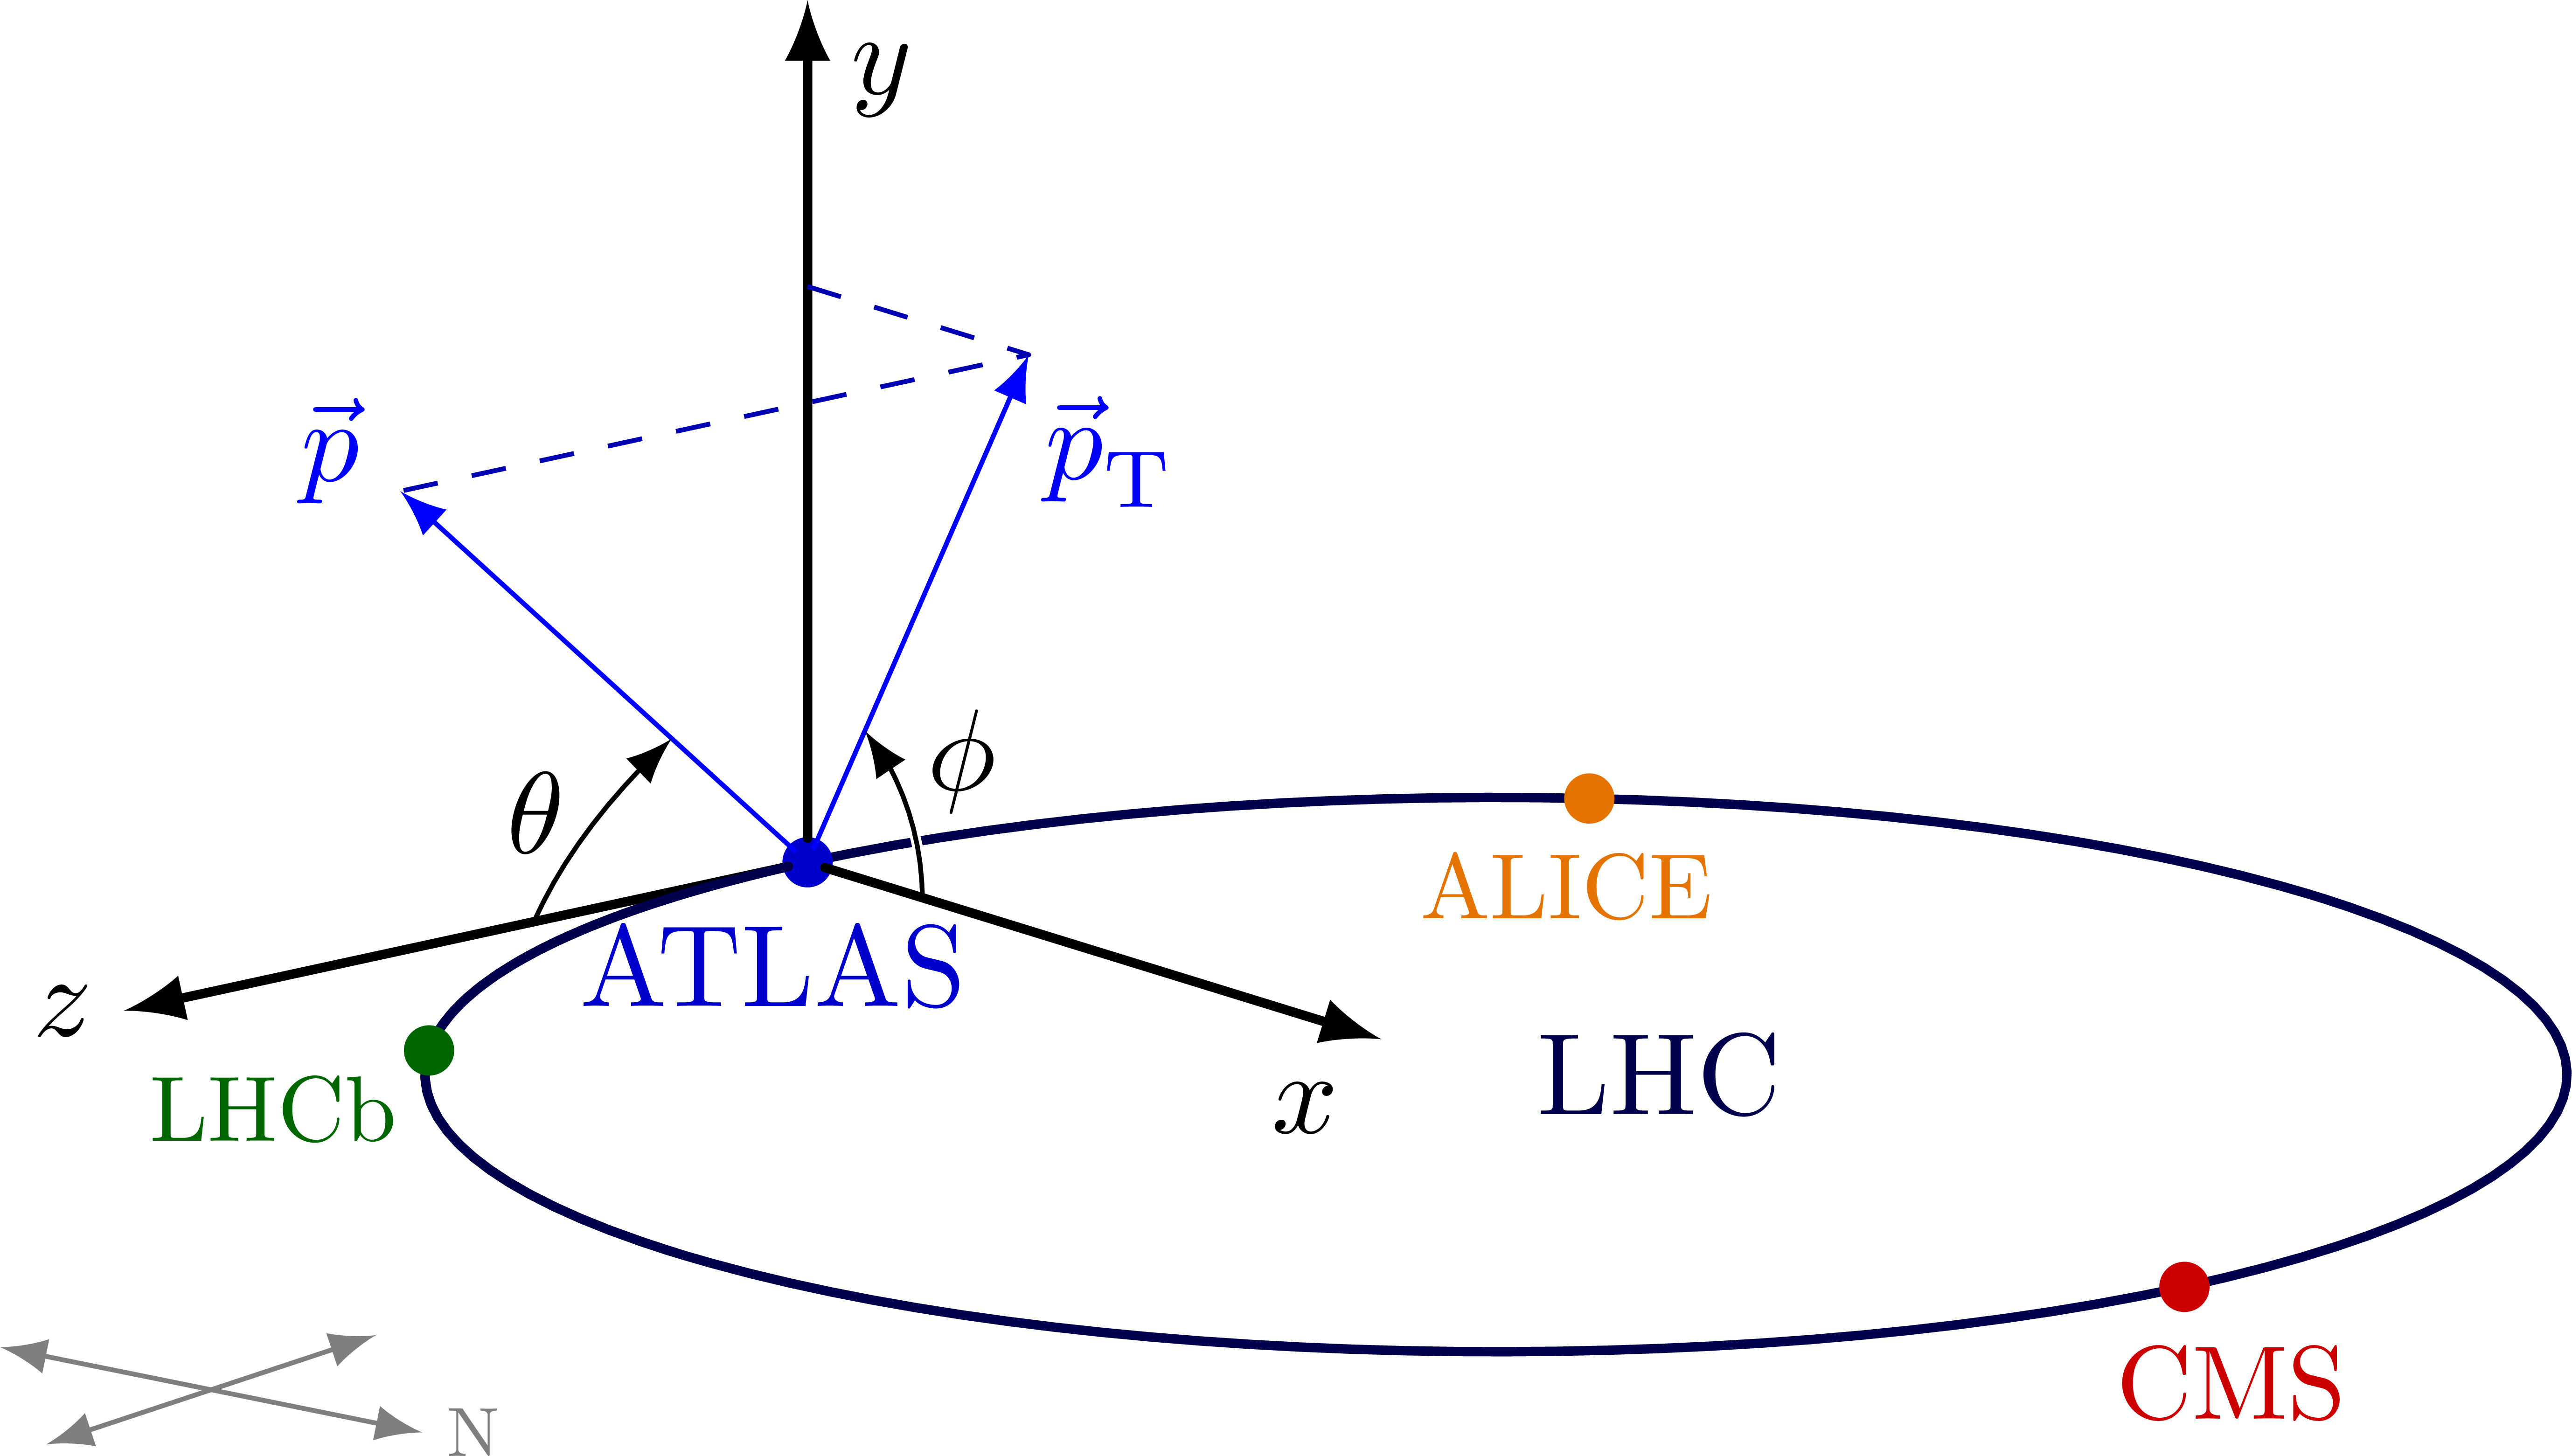
\includegraphics[width=0.6\textwidth]{images/ATLAS_Coordinate_System.png}
    \caption{Diagram showing the orientation of the coordinate system used in ATLAS as well as relevant kinematic 
    variables.}
    \label{fig:ATLAS_Coordinate_System}
\end{figure}

\subsection{Inner Tracking Detector}

The core of the ATLAS detector \cite{atlas-detector} is the inner tracking detector, which is primarily responsible 
for precisely measuring the trajectories of charged particles by recording currents from electrons freed via the 
ionization of detector material. It is a combination of three different sub-systems: a pixel detector on the inside 
surrounded by a semiconductor tracker (SCT) and finally a transition radiation tracker (TRT) on the outside. The pixel 
detector and SCT are built from silicon wafers while the TRT is made up of drift tubes filled with a Xenon-based gas 
mixture, with each subsequent part of the detector providing increasingly less granular position measurements. 
Geometrically the inner detector consists of barrel and endcap components where the barrel is a cylinder surrounding 
the beam and the endcaps are disks placed on either side of the barrel to detect forward particles within 
$|\eta| < 2.5$. \par

\begin{figure}
\centering
    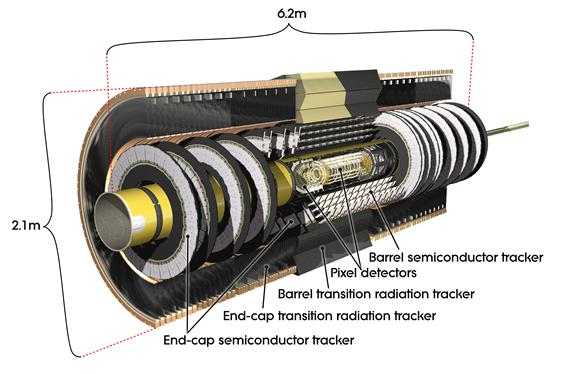
\includegraphics[width=0.8\textwidth]{images/ATLAS_Inner_Detector.png}
    \caption{Schematic of the ATLAS inner detector and its components from \cite{atlas-run3-setup}.}
    \label{fig:ATLAS_Inner_Detector}
\end{figure}

The pixel detector \cite{pernegger-pixel-detector} is silicon-based and made up of 92 million individual sensor 
elements (pixels) arranged in 4 layers for the barrel component (1736 modules total) as well as 3 disk layers for each 
endcap (288 modules total). The innermost layer, called the insertable B-layer \cite{atlas-insertable-b-layer}, was 
inserted prior to run 2 of the LHC and is located a distance of $33mm$ from the beam pipe. It has the smallest individual 
pixel elements at $50\times250\ \mu m^2$, allowing for increased position resolution closest to the beam. The remaining 
layers have pixels of size $50\times400\ \mu m^2$, resulting in an overall spatial resolution of $\sim 8 \mu m$ in 
$r\phi$ and $\sim 75 \mu m$ in $z$. All pixel sensors have a thickness of $250 \mu m^2$. Individual sensor elements 
are not arranged end to end but rather partially overlap to ensure complete $\phi$ coverage of each layer. The final 
layer of the pixel detector is located at $122.5mm$ from the beam. \par

Surrounding the pixel detector is the semiconductor tracker (SCT) \cite{atlas-sct}, which is similar in design and 
functionality, but contains larger silicon-based detector elements (strips). It is made up of 4 barrel layers (2112 
modules total) and 9 disk layers for each endcap (1976 modules total) starting at $299mm$ from the beam for the first 
barrel layer and ending at $514mm$ for the last. In total, the SCT contains over 6 million strips with a 
pitch\footnote{Pitch in this context refers to the distance between the center of adjacent detector elements} of 
$80\mu m$ and a length of $12cm$. To combat the decrease in resolution from the increased size of the strips compared 
to pixels, individual strips are rotated relative to each other on either side of a sensor module. \par

The final sub-system of the inner detector is the transition radiation tracker (TRT) \cite{atlas-trt}, which differs 
quite significantly in design from the other two components. It consists of 300,000 gas filled drift tubes (or straws) 
with a thin wire at the center, each with a diameter of $4mm$. There are 50,000 straws of $144cm$ around the length of 
the barrel arranged parallel to the direction of the beam and extending outward to $1082mm$ from the beam line. A 
further 250,000 straws of $39cm$ pointing outward radially from the beam are located in the two endcaps. In addition to 
ionization, charged particles passing through the TRT also emit transition radiation from crossing a boundary between 
two mediums with different dielectric constants. Since the amount of emitted radiation is inversely proportional to the 
mass of the particle crossing the boundary, the TRT can be used to discriminate between electrons and heavier charged 
particles such as pions. This gives it a unique advantage over the other inner detector sub-systems, although it comes 
at the cost of loss of measurement information along the longitudinal direction of the straws. \par

As mentioned before, the combination of these three sub-systems is mainly responsible for precise measurements of 
particle trajectories and momenta while minimally affecting their energies. This is accomplished by the presence of 
nearly 100,000,000 finely segmented individual readout channels spread across pixels, strips and straws. Overall, the 
inner detector achieves a momentum resolution of at least
\begin{equation}
\sigma_{pT}/p_T = 0.05\% p_T \oplus 1\%
\end{equation}
where $\oplus$ denotes an addition in quadrature. Momentum resolution generally worsens with increasing particle 
momentum due to the comparatively less pronounced curvature of high momentum tracks.

\subsection{Electromagnetic and Hadronic Calorimeters}

Surrounding the inner tracking detector of ATLAS is an extensive calorimeter system made up of both hadronic and 
electromagnetic sampling calorimeters. The purpose of these components is to stop incoming particles, making them 
deposit their energy to facilitate precise energy measurements as well as particle identification for photons, 
electrons and hadrons. To accomplish this, sampling calorimeter elements are made up of alternating layers of an 
absorbing material and an active material. The absorber is meant to be dense, triggering interactions with incoming 
particles which leads to particle showers\footnote{A particle shower is a cascade of particles produced in an 
interaction with detector material}. Electromagnetic showers proceed via repeated instances of bremsstrahlung and 
$e^+e^-$ pair creation triggered by a single photon, electron or positron. Hadronic showers start with a break up of 
the incoming hadron (both charged and neutral), evolve into further interactions and usually also contain an 
electromagnetic component. Each section of active material then captures information about the energy of a shower 
via ionization or scintillation\footnote{These parts of the calorimeter are functionally identical to a tracking 
detector} from charged particle interactions. This process repeats through the layers of the calorimeter until all of 
the energy is deposited. The ATLAS calorimeter system uses two different technologies: a Liquid Argon (LAr) 
calorimeter on the inside and a Tile calorimeter on the outside. \par

\begin{figure}
\centering
    \includegraphics[width=0.8\textwidth]{images/ATLAS_Calorimeter.png}
    \caption{Schematic of the ATLAS calorimeters and their components from \cite{atlas-run3-setup}.}
    \label{fig:ATLAS_Calorimeter}
\end{figure}

The inner LAr calorimeter system has both electromagnetic and hadronic components (as well as a separate forward 
calorimeter). Each of these uses Liquid Argon as the active material with different absorbers. The electromagnetic 
calorimeter covers all of the barrel as well as the interior section of the endcaps and uses lead to stop photons and 
electrons up to a radiation length of $24X_0$\footnote{$X_0$ denotes the average length an electron needs to travel 
in material to reduce its energy by $1/e$}. The hadronic and forward components of the LAr calorimeter are 
restricted to the endcaps only and use copper and tungsten as absorbers respectively to capture forward hadrons up to 
$|\eta| < 4.9$. While hadrons lose part of their energy in the electromagnetic calorimeter, this is usually not enough 
to stop them completely. Because of this, the tile calorimeter, which is made out of steel and plastic scintillator, 
surrounds the LAr components in their entirety, providing a full hadronic calorimeter outside of the LAr endcaps. The 
energy resolution differs between these individual components as

\begin{equation} % EM calorimeter
(\sigma_{E}/E)_{EM} = 10\% / \sqrt{E} \oplus 0.7\%
\end{equation}

\begin{equation} % hadronic calorimeter for barrel and endcap, not forward
(\sigma_{E}/E)_{Had} = 50\% / \sqrt{E} \oplus 3\%
\end{equation}

\begin{equation} % hadronic calorimeter for forward
(\sigma_{E}/E)_{Fwd} = 100\% / \sqrt{E} \oplus 10\%
\end{equation}

\subsection{Muon Spectrometer}

The only remaining charged particles that reliably penetrate the electromagnetic and hadronic calorimeters are muons. 
Though inherently unstable, their relatively long lifetimes of $2.20\times10^{-6}\ s$ ensure they mostly don't decay 
within the detector at energies commonly seen in LHC collisions. They also generally do not interact significantly 
with detector material, allowing them to keep comparatively straight trajectories as they travel outward. As such, 
the outermost part of the ATLAS detector is a muon spectrometer used to identify muons and measure their momenta. 
The muon spectrometer consists of 2 main parts made up of 5 different detector technologies. The first is a precision 
detector made up of 380,000 Monitored Drift Tubes (MDTs) which provide precision measurements on muon momenta with 
a resolution of

\begin{equation} % at pT = 1 TeV
\sigma_{pT}/p_T = 10\%
\end{equation}

These tubes are filled with a gas mixture and measure ionizing radiation (similar to the inner detector). The second 
component is a system of fast-response detectors made up of Resistive Plate Chambers (RPCs), Thin Gap Chambers (TGCs), 
Micromegas and Small-Strip Thin-Gap Chambers (sTGCs) which work together to provide rapid muon identification. All of 
these use similar technologies to the MDTs but are optimized for speed rather than precision. \par

%https://link.springer.com/chapter/10.1007/978-3-030-52877-5_3
\begin{figure}
\centering
    \includegraphics[width=0.6\textwidth]{images/ATLAS_Muon_Spectrometer.png}
    \caption{Schematic of the ATLAS muon spectrometer from \cite{atlas-run3-setup}.}
    \label{fig:ATLAS_Muon_Spectrometer}
\end{figure}

\subsection{Magnet System}

As previously discussed, making measurements of charged particle momenta relies on identifying the curvature of their 
trajectory in an applied magnetic field. Stronger fields provide more curved trajectories which improve momentum 
resolution, especially for high $p_T$ particles. In addition to the magnet system present in the LHC, which is 
responsible for the acceleration of the proton beams, the ATLAS detector has its own integrated magnet system 
(figure \ref{fig:ATLAS_Magnets}). The core of this is a solenoidal magnet around the inner detector, which applies a 
uniform $2T$ magnetic field along the direction of the beam. This means charged particles traveling from the collision 
point will follow helical trajectories with a pitch determined by their transverse momentum $p_T$ inside the inner 
detector. In addition to the interior solenoid there are three toroidal magnet systems made up of 8 coils each, one 
around the barrel portion of the detector and one around each of the end-caps. These provide a circular magnetic field 
up to $3.5T$ in the outer parts of the detector used to deflect the trajectories of muons for more accurate momentum 
measurements in the muon spectrometer. \par

%https://link.springer.com/chapter/10.1007/978-3-030-52877-5_3
\begin{figure}
\centering
    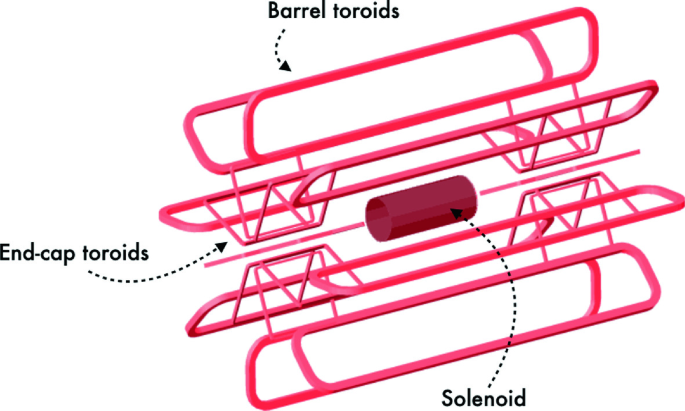
\includegraphics[width=0.6\textwidth]{images/ATLAS_Magnets.png}
    \caption{Schematic of the ATLAS magnet system.}
    \label{fig:ATLAS_Magnets}
\end{figure}

\subsection{Trigger and DAQ}

The LHC provided bunch crossing rate of up to 40 MHz floods the ATLAS detector with data in excess of what can 
realistically be recorded and stored. Much of this data comes from collision events likely to contain little of 
interest to a physicist on the ATLAS experiment\footnote{For example, events where no "hard scatter" collision 
takes place (i.e. pile-up events)}. To combat this, decisions need to be made about whether individual events are 
worth recording and storing, which is the responsibility of the ATLAS Trigger and Data Acquisition (DAQ) systems. For 
run 3, the combined effect of all experimental triggers reduces the frequency of recorded events from 40 MHz to 
around 3 kHz \cite{oliveiradamazio-trigger}. This is accomplished with two sequentially applied systems: the Level-1 
Trigger (L1) and the High Level Trigger (HLT). \par

\begin{figure}
\centering
    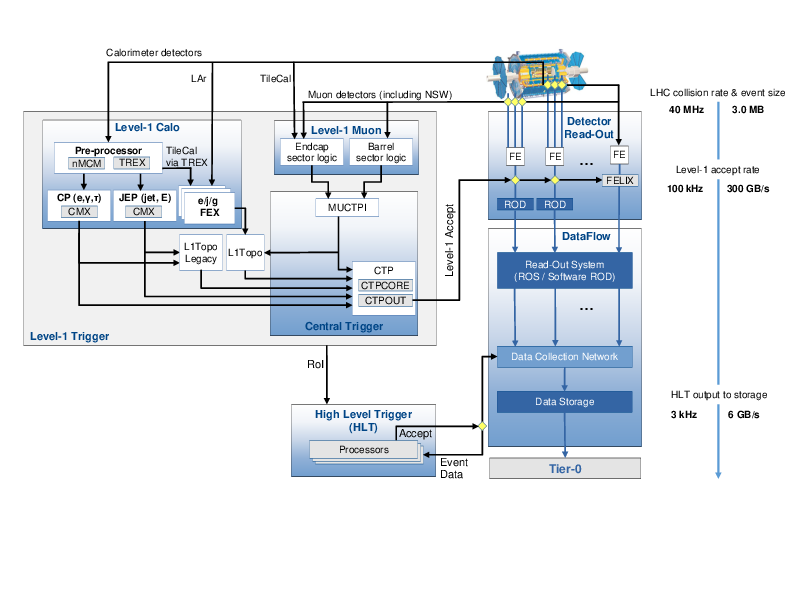
\includegraphics[width=0.8\textwidth]{images/Trigger_System.png}
    \caption{Diagram showing the core components of the ATLAS Trigger and DAQ from \cite{atlas-run3-setup}.}
    \label{fig:Trigger_System}
\end{figure}

The L1 trigger is a hardware trigger that filters events by identifying large energy deposits in the calorimeter 
(L1-Calo) as well as high $p_T$ muons in the fast-response muon system (L1-Muon). The Central Trigger Processor (CTP) 
then records events based on both individual hardware triggers as well as their combination via computation of the 
pairwise invariant masses of muons and energy clusters in the calorimeter (L1-Topo). Events passing L1 undergo a 
lightweight version of the object reconstruction chain and get passed through the HLT, where a set of more complex 
criteria are applied to reduce the number of events further. The details of this require knowledge of the object 
reconstruction chain, which is discussed in the next section.

\section{Object Reconstruction}

Having spent some time familiarizing ourselves with the detector hardware, it is important to highlight how 
measurements are transformed into physical quantities such as particle trajectories, momenta and energies. This 
will allow us to approach the answer to the question of how Higgs bosons are identified in complex proton-proton 
collision events at the LHC. The core of this is the trajectory reconstruction itself, which combines individual 
measurements in the inner detector into physical particle tracks. Energy deposits in the calorimeter are also 
clustered and matched with the tracks in an attempt to isolate individual contributions. With this fundamental 
information, certain particles (such as electrons, photons and muons) can be directly identified and particle jets 
created by the hadronization of quarks can be reconstructed. Some parts of reconstruction are performed initially 
at the level of the HLT\footnote{Often times with some approximations or faster, less accurate algorithms} (online) 
while others are only done once after an event is recorded (offline). Furthermore, given the prevailing use of Monte 
Carlo simulated events in finetuning reconstruction strategies, careful checks have to be completed to ensure 
parity in performance between simulation and data. This chapter outlines all of these aspects of object 
reconstructions in detail to give a complete picture of the low level physics objects relevant to measurements of 
physical processes in the ATLAS detector. \par

\subsection{Fundamental Objects: Tracks, Clusters and Vertices}

The first step in the ATLAS reconstruction chain is identifying trajectories of particles passing through the 
inner detector \cite{cornelissen-tracking}. Specifically we are interested in reconstructing a set of parameters 
given by $(d_0, z_0, \phi, \theta, \frac{q}{p})$ shown in figure \ref{fig:Impact_Parameters} from individual energy 
deposits ("hits") in the detector. The transverse and longitudinal impact parameters (IP) $d_0$ and $z_0$ are 
defined to be the coordinates of the point of closest approach between a track and the primary interaction point 
when the track is fully extrapolated in both directions. This functions as a measure of whether a track is likely 
to have originated from the primary interaction point (small IP) or from some later decay or interaction or pile-up 
(large IP). The other 3 tracking variables are previously discussed representations of the particle 4-vector. \par

%https://indico.nbi.ku.dk/event/758/attachments/1684/2344/trackingnote.pdf
\begin{figure}
\centering
    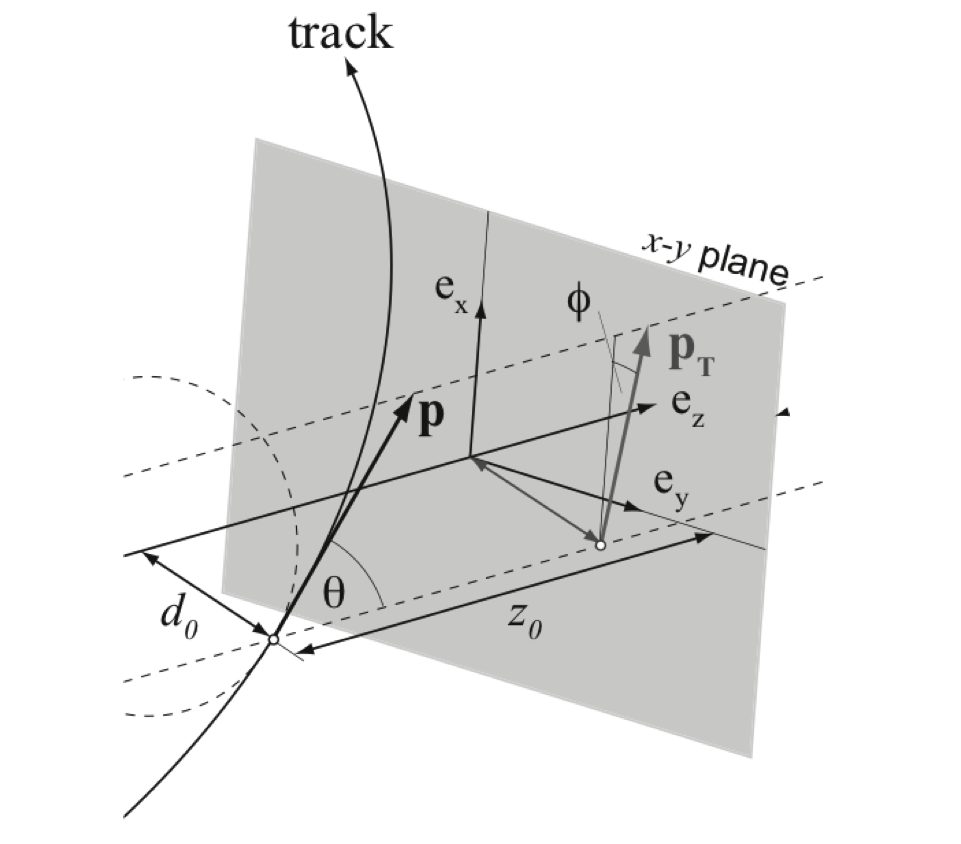
\includegraphics[width=0.8\textwidth]{images/Impact_Parameters.png}
    \caption{Diagram visualizing track parameters used in ATLAS.}
    \label{fig:Impact_Parameters}
\end{figure}

Tracking begins with a process called spacepoint formation, which clusters adjacent hits reaching some energy 
threshold in each layer of the pixel and SCT detectors. These clusters are transformed into global coordinates 
representing individual intersection points between particle trajectories and detector material. Spacepoints in 
subsequent layers are then grouped into batches of 3 to create track seeds. This is preferentially done in the SCT 
due to the lower density of spacepoints, but pixel seeds are also considered. Each seed is required to meet specific 
quality criteria based on rough estimates of track paramters to minimize the presence of duplicate seeds for a given 
track and reduce computational overhead. The remaining seeds are then extended in both directions via a track 
finding algorithm based on the combinatorial Kalman filter (CKF) \cite{fruehwirt-kalman-filter}. This algorithm 
repeatedly adds compatible clusters on adjacent layers to a track candidate and smoothes the estimated trajectory 
taking into account detector resolution effects. In the case where multiple compatible spacepoints are found, 
diverging track candidates are created and extended separately. Additionally, a prodedure called Bremsstrahlung 
recovery allows seeds that fail the track finding step entirely to be considered with a decreased quality threshold. 
This procedure is triggered when a failed seed is matched to an interesting region in the calorimeter, which helps 
recover performance for electron tracks radiating photons via Bremsstrahlung as they traverse the detector. \par

Once the full set of track candidates is established via the CKF, an ambiguity resolution stage attempts to remove 
all fake and duplicate tracks by enforcing a more stringent set of quality criteria. Tracks with a significant 
amount of overlapping (shared) hits are compared against each other and only the highest quality track is retained. 
However, due to the dense tracking environment of ATLAS (particularly in the pixel detector), a limited number of 
shared hits between tracks is allowed. A dedicated algorithm is used to perform cluster splitting 
\cite{atlas-cluster-splitting}, which aims to split clusters consisting of multiple particles into their individual 
components. After ambiguity resolution, a $\chi^2$ fit is performed on the remaining candidates for a final track 
parameter estimate. Where applicable, an attempt is made to extend track candidates made from pixel and SCT hits 
into the TRT via another Kalman filter based algorithm. These extensions are only retained if the overall $\chi^2$ 
fit of a track does not worsen with the additional TRT hits. Aside from this forward tracking procedure, a 
secondary back-tracking pass is done to increase reconstruction efficiency of particles produced further from the 
beam. This procedure is mostly identical to forward tracking, but starts by searching for hit segments in the TRT 
aligned with regions containing significant energy deposits in the calorimeter. Seeds are then created in layers 
of the pixel and SCT detectors consistent with these TRT segments using two spacepoints only. \par

Energy deposits in the calorimeter are also grouped (into so called topo-clusters) using a dedicated clustering 
algorithm and then split to reflect the presence of multiple particle contributions where applicable\footnote{This 
happens when deposits are topologically close to each other but contain multiple separable energy peaks}. For many 
practical applications tracks and calorimeter clusters are matched to each other via an algorithm called "Particle 
Flow" \cite{atlas-pflow} or a modification thereof. In particular, "Particle Flow" estimates the energy contribution 
of a charged particle track to a topo-cluster to isolate the neutral contributions. This results in a unified 
description of neutral and charged particles in the detector defined by a combination of information from tracks and 
topo-clusters. \par

The presence of a significant amount of pile-up interactions (as shown in figure \ref{fig:Luminosity_vs_Pileup}) 
necessitates identifying tracks from the primary interaction of interest (i.e. the "hard scatter" collision) and 
separating them from the rest of the event. This is accomplished via primary vertex reconstruction through an 
algorithm made up of a vertex finding and a vertex fitting component \cite{atlas-vertex-reconstruction}. The 
process begins by considering all tracks above a minimum $p_T$ threshold and within a certain impact parameter 
window in order to limit contributions from fake tracks, pile-up and secondary interactions to the position of 
the primary vertex. A vertex seed is created centered at the beam-spot in the transverse plane and the mode of the 
z-position of all tracks passing the requirements. This seed is used as the starting point for an iterative $\chi^2$ 
minimization, which iteratively assigns a weight reflecting compatibility with the current vertex position to each 
track and then recalculates the vertex position based on this weight. Once this minimization converges, all tracks 
with a sufficient compatibility to the final vertex position are removed from the pool and the process is repeated. 
After all vertices are found, the vertex with the largest $\Sigma p_T^2$ is marked as the primary vertex. \par

\begin{figure}
\centering
    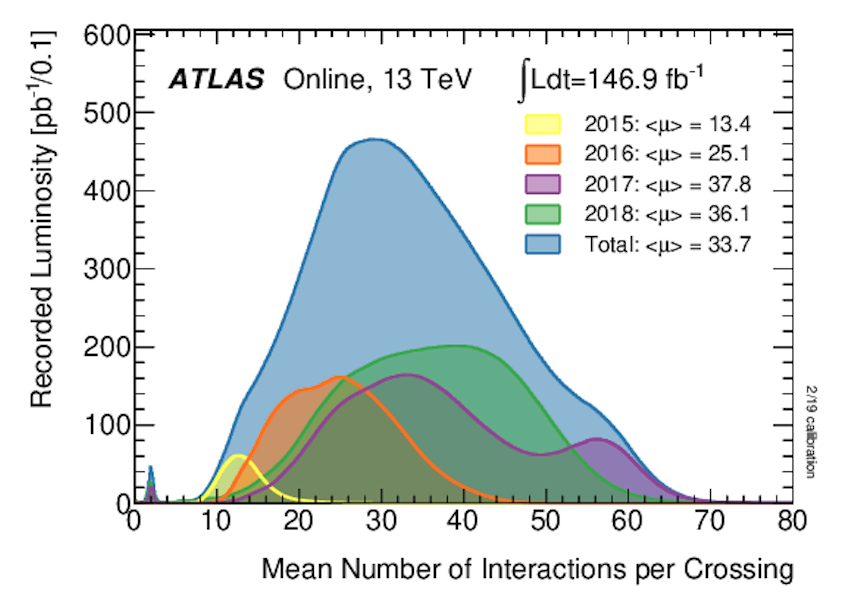
\includegraphics[width=0.8\textwidth]{images/Luminosity_vs_Pileup.png}
    \caption{Recorded luminosity vs average number of pile-up interactions for each run from 
    \cite{atlas-run3-setup}.}
    \label{fig:Luminosity_vs_Pileup}
\end{figure}

\subsection{Photons}

\subsection{Electrons}

\subsection{Muons}

\subsection{Hadronic Taus}

\subsection{Quarks, Hadrons and Missing Energy}